\documentclass[11pt,a4paper]{article}

\usepackage[utf8]{inputenc}
\usepackage[T1]{fontenc}
\usepackage[margin=2.5cm]{geometry}
\usepackage{amsmath,amssymb}
\usepackage{booktabs}
\usepackage{tabularx}
\usepackage{enumitem}
\usepackage{xcolor}
\usepackage{tikz}
\usetikzlibrary{positioning,arrows.meta,shapes.geometric,fit}
\usepackage[hidelinks]{hyperref}

% long identifiers in \texttt cannot hyphenate: allow looser lines instead of overfull ones
\setlength{\emergencystretch}{3em}
\sloppy

\definecolor{critic}{RGB}{160,40,40}
\definecolor{resolved}{RGB}{30,110,60}
\definecolor{rule}{RGB}{30,90,160}

% Open critical remark: a weakness that remains after the implementation.
\newenvironment{critique}[1]{%
  \par\medskip\noindent\textbf{\color{critic}Open critique -- #1.}\ }{\par\medskip}
% A critique of the first version and how it was solved.
\newenvironment{resolved}[1]{%
  \par\medskip\noindent\textbf{\color{resolved}Resolved -- #1.}\ }{\par\medskip}
% An adopted modelling rule.
\newenvironment{adopted}[1]{%
  \par\medskip\noindent\textbf{\color{rule}Rule #1.}\ }{\par\medskip}

\newcommand{\Mset}{\mathcal{M}}
\newcommand{\Oset}{\mathcal{O}}
\newcommand{\Jset}{\mathcal{J}}
\newcommand{\Uset}{\mathcal{U}}
\newcommand{\Info}{\mathcal{I}}
\newcommand{\cin}{c^{\mathrm{in}}}
\newcommand{\cout}{c^{\mathrm{out}}}
\newcommand{\sch}{\mathrm{sch}}
\newcommand{\bd}{\mathrm{bd}}
\newcommand{\EST}{\mathrm{EST}}
\newcommand{\RE}{\mathrm{RE}}
\newcommand{\code}[1]{\texttt{#1}}

\title{Machine Unavailability in the Blocking FJSP:\\
Two Graph Representations, their Implementation and a Critical Assessment}
\author{Mariana Correia}
\date{\today}

\begin{document}
\maketitle

\begin{abstract}
This document specifies the machine-unavailability constraint added to the blocking
flexible job shop (FJSP with finite input and output buffers), and two ways of exposing it to a
graph neural network policy: (A) features on the existing machine nodes and action edges and
(B) dummy operations. A first version of this document criticised the proposal on seven
points. They are now resolved in the implementation
(\code{src/env\_unavailability.py} and related modules):
(1) both representations are built from one function and carry exactly the same information;
(2) the ``stand-by'' feature is renamed \emph{planned downtime};
(3) every interaction with blocking has an explicit rule, shared by the environment, the
CP-SAT reference and the constraint checks;
(4) the new features use a fixed scale instead of per-state min--max;
(5) nothing the policy, its mask or its look-ahead sees depends on future breakdowns;
(6) machines have heterogeneous reliability and a failure rate that grows with age (Weibull,
$\beta>1$); and
(7) BOPO uses common random numbers, and the reference under breakdowns is reported as a
clairvoyant bound.
The remaining open critiques are kept, with a calibration result that matters for the thesis: a
greedy dispatching rule gains almost nothing from knowing the windows, so any benefit of a
representation must come from look-ahead learned by the policy.
\end{abstract}

\tableofcontents

%=======================================================================
\section{Scope}
%=======================================================================

The thesis compares graph representations of the FJSP under industrial constraints. The
blocking constraint was represented in two structurally different but information-equivalent
ways (a \code{buffer} node type, \code{ojmb}, and buffers as dummy machines, \code{ojmd}),
plus a representation-blind control (\code{ojm\_blk}) on the same dynamics.
Machine unavailability is the next constraint, and it is \textbf{always combined with blocking}:
every instance has the buffers of the blocking study ($\cin=2$, $\cout=1$), and the windows are
added on top.

An \emph{unavailability window} is a time interval during which a machine cannot start an
operation. Two sources are modelled:
\begin{itemize}[nosep]
  \item \textbf{Scheduled windows} (planned maintenance): known from $t=0$.
  \item \textbf{Breakdowns}: random, and revealed only when they happen.
\end{itemize}
Three representations are compared, all on the blocking graph with buffer nodes (\code{ojmb}):
\begin{center}
\begin{tabular}{@{}lll@{}}
\toprule
Code name & Representation & Environment class \\
\midrule
\code{ojmb\_uf} & A: features on machines and action edges & \code{FJSPEnvUnavailFeatures} \\
\code{ojmb\_uo} & B: dummy operations & \code{FJSPEnvUnavailDummyOps} \\
\code{ojmb\_u0} & control: window-blind graph, same dynamics & \code{FJSPEnvUnavailBlind} \\
\bottomrule
\end{tabular}
\end{center}
A mode (\code{scheduled}, \code{breakdown} or \code{mixed}) selects which sources are active.

%=======================================================================
\section{Problem definition}
%=======================================================================

\subsection{Blocking FJSP}

Let $\Jset$ be the jobs, $\Oset$ the operations and $\Mset$ the machines, with processing time
$p_{om}>0$ if machine $m$ is eligible for operation $o$. Each machine $m$ has an input buffer of
capacity $\cin$ and an output buffer of capacity $\cout$. A part moves from the input buffer of
$m$ to $m$, then to the output buffer of $m$, and then to the input buffer of its next machine.
A routing $(j,m)$ is legal while the input buffer of $m$ has a free slot, and machines process
their input buffer in FIFO order. A finished part that finds the output buffer full stays on
the machine, which is then \emph{blocked}. A circular wait is resolved by a \emph{swap}, and a
one-step look-ahead masks routings that lead to a deadlock. The environment is event-driven,
with a clock $t$ that only moves forward.

\subsection{Unavailability windows}

For every machine $m$ let $\Uset_m=\{w=(s_w,e_w,\tau_w)\}$, with $\tau_w\in\{\sch,\bd\}$, be a
sorted list of pairwise disjoint, half-open windows $[s_w,e_w)$ with integer times. The windows
of an episode (its \emph{scenario}) are sampled once when the episode is reset
(Section~\ref{sec:breakdowns}), or read from the instance for the stored validation and test
sets. No random number is drawn while the episode runs.

\subsection{Adopted rules, including the interaction with blocking (point 3)}
\label{sec:rules}

Each rule is implemented once and used identically by three components: the environment
(\code{src/env\_unavailability.py}), the CP-SAT reference (\code{src/solver\_blocking.py}), and
the independent schedule checks (\code{src/metrics/unavailability.py}).

\begin{adopted}{R1 (no start inside a window)}
An operation never starts at a time $x$ with $s_w\le x<e_w$.
\end{adopted}

\begin{adopted}{R2 (scheduled windows are non-preemptive)}
An operation that starts before a scheduled window must fit before it with its nominal time:
$x<s_w \Rightarrow x+p_{om}\le s_w$. Otherwise it waits until $e_w$. The earliest admissible
start is
\[
  \EST_m(r,p)=\min\{x\ge r:\ \text{R1 holds, and } x+p\le s_w \text{ for every scheduled } w
  \text{ with } x<s_w\}.
\]
\end{adopted}

\begin{adopted}{R3 (breakdowns are preempt-resume)}
The running part stays on the machine and continues after the repair, so its end is
\[
  C=\mathrm{resume}(x,p)=x+p+\sum_{w\text{ met}}(e_w-s_w),
\]
where a window is \emph{met} when processing, extended by the earlier windows, reaches $s_w$.
A breakdown can push an operation into a later scheduled window, which then pauses it as well.
\end{adopted}

\begin{adopted}{R4 (routing into a machine that is down is allowed)}
Legality stays purely capacity-based. A part may enter the input buffer of a machine that is
down, and it waits there. This is deliberate: if such routings were masked, the policy could
never make the mistake the representations are supposed to help it avoid. The constraint
would then live in the mask, and the comparison between A and B would measure noise.
\end{adopted}

\begin{adopted}{R5 (unloading continues)}
A window stops only \emph{starts}, and, for a breakdown, the progress of the running part.
A part in the output buffer, or a finished part held on a blocked machine, may leave when its
next operation is routed, because moving a finished part is not processing. In CP-SAT, this is
why the machine occupancy interval $[s,d]$ (which includes holding) is not blocked by windows.
\end{adopted}

\begin{adopted}{R6 (blocked and down are independent)}
A machine's status is a pair (blocked or not, available or not). When the held part of a
blocked machine leaves during a window, the machine still cannot start its queue head
before the window ends.
\end{adopted}

\begin{adopted}{R7 (swaps and waits)}
A swap requires every machine of the cycle to start its queued part at once, because that start
frees the slot the predecessor's part moves into. A machine that is down, or whose queue head
would cross a planned maintenance, cannot do this, so it is excluded from swap cycles. If no
cycle remains, the state is a \emph{wait}, not a deadlock: the clock jumps to the earliest time
one of those machines can start (counted in \code{num\_waits}).
\end{adopted}

\begin{adopted}{R8 (event clock)}
The clock moves to the next of three kinds of event: a processing completion; the time an idle
machine with a queue can start (the end of its window); or, in a wait, the time a blocked
machine can. The loop is:
\begin{enumerate}[nosep]
  \item start every idle, unblocked machine whose queue head satisfies R1--R2 at $t$, with end
        $\mathrm{resume}(t,p)$ on the true windows;
  \item if every job is done, or some routing is legal, stop: a decision is needed;
  \item if a completion or a pending start exists, move $t$ to the earliest one, complete the
        operations that end then, and go to 1;
  \item otherwise, if a swap cycle exists among the machines that can start (R7), swap and go to 1;
  \item otherwise, move $t$ to the earliest time a blocked machine can start (a wait), and go to 1.
\end{enumerate}
\end{adopted}

\subsection{Information model (point 5)}
\label{sec:info}

The dynamics run on the true windows. What may be \emph{known} at time $t_0$ is the
\emph{information view} $\Info(t_0)$ (\code{information\_view}): every scheduled window, every
breakdown that has ended, and, for a breakdown in progress, only an estimated end
$t_0+\mathrm{MTTR}_m$ (Section~\ref{sec:breakdowns}). Breakdowns that start after $t_0$ are not
in the view. Four mechanisms keep the future out of reach:
\begin{enumerate}[nosep]
  \item \textbf{Graph features and projections.} The machine free time, the projected end of
        every routed part, and job readiness are computed from $\Info(t)$. For a running part the
        policy sees $\mathrm{resume}(x,p)$ on the view, not the true end: that may already
        include a future breakdown (\code{\_known\_end}).
  \item \textbf{Deadlock look-ahead.} The one-step simulation that masks deadlocking routings
        runs on $\Info(t_0)$ (\code{\_lookahead}), and the running parts end where the view says.
        A routing is never masked because of a breakdown that has not happened.
  \item \textbf{Mask ranking.} The top-$k$ earliest-completion ranking of the action mask is
        \emph{window-blind}, and identical for every representation. The mask therefore carries
        no window information, and all of it must arrive through the graph. Before this change,
        a window-aware mask would have given most of the information to the ``blind'' control too.
  \item \textbf{Teacher.} The imitation teacher of the warm start is the window-aware
        earliest-completion rule on $\Info(t)$, the same for every representation.
\end{enumerate}
Two tests enforce this.
\begin{itemize}[nosep]
  \item \code{test\_no\_information\_leak}: it removes every future breakdown, lengthens the
        repair in progress, adds a new future breakdown, and checks that the state, the mask and
        the teacher's choice are unchanged.
  \item \code{test\_same\_dynamics\_and\_mask\_for\_every\_representation}: it checks that the
        three representations produce the same masks and the same schedule for the same actions.
\end{itemize}

%=======================================================================
\section{Breakdown model: heterogeneous reliability and increasing failure rate (point 6)}
\label{sec:breakdowns}
%=======================================================================

The first version modelled breakdowns as ``totally random''. If every machine fails at the same
constant rate, no state feature predicts the next failure. The policy can then only react, and
after a failure A and B hold the same information, so a null result would be expected and
uninformative. The adopted model gives the representations something to learn.

\paragraph{Time to failure.} For machine $m$ the time to failure $T$ is Weibull with shape $\beta$
and scale $\eta_m$, with survival function, hazard rate and conditional failure probability
\begin{align*}
  R(a)&=e^{-(a/\eta_m)^\beta},\qquad
  h(a)=\frac{\beta}{\eta_m}\Bigl(\frac{a}{\eta_m}\Bigr)^{\beta-1},\\
  P_m(H\mid a)&=1-\frac{R(a+H)}{R(a)}
  =1-\exp\Bigl[\Bigl(\frac{a}{\eta_m}\Bigr)^{\beta}-\Bigl(\frac{a+H}{\eta_m}\Bigr)^{\beta}\Bigr],
\end{align*}
where $a$ is the machine's \emph{age}. With $\beta=2>1$ the hazard grows with age (wear-out):
an old machine is more likely to fail soon, and the age is informative. With $\beta=1$
(exponential) $P_m(H\mid a)$ would not depend on $a$.

\paragraph{Heterogeneous reliability.} For each machine an availability
$A_m\sim U(0.75,0.90)$ and a mean repair time $\mathrm{MTTR}_m\sim U(0.06,0.12)\cdot LB$ are
drawn. $LB$ is the instance's solver-free makespan lower bound, so every length scales with the
instance. The scale follows from
\[
  \mathrm{MTBF}_m=\mathrm{MTTR}_m\,\frac{A_m}{1-A_m},\qquad
  \eta_m=\frac{\mathrm{MTBF}_m}{\Gamma(1+1/\beta)}.
\]
Some machines are therefore systematically less reliable than others. Combined with the age,
this is a signal a policy can learn to use (route away from an old, unreliable machine).

\paragraph{Repair and renewal.} Repair times are exponential with mean $\mathrm{MTTR}_m$.
Because the exponential distribution is memoryless, the expected remaining repair is
$\mathrm{MTTR}_m$ however long the machine has been down: this is the estimate the view uses.
A repair and a planned maintenance both renew the machine (age~$0$).

\paragraph{Sampling.} Windows are sampled machine by machine over $[0,5\,LB]$. From the last
renewal, a failure time is drawn. If a planned maintenance starts first, the machine is renewed
at its end and a new failure time is drawn. A repair that would overlap a maintenance is cut
short (the maintenance takes over), so windows never overlap. Scheduled windows are 0--1 per
machine plus one extra on the most loaded machine (the bottleneck, found from the loads, not
from machine indices), each $0.05$--$0.12\,LB$ long. The same seed gives the same planned
maintenance in \code{scheduled} and \code{mixed} mode.

%=======================================================================
\section{Representation A: features on existing nodes and edges}
\label{sec:repA}
%=======================================================================

\subsection{Definition (points 1 and 2)}

A single method, \code{\_window\_information()}, is the analogue of
\code{\_buffer\_information} in the blocking study. For each machine $m$ it returns:
\begin{itemize}[nosep]
  \item its \emph{current} window (the one containing $t$) and its \emph{next} known window
        starting within the horizon $H=0.5\,LB$, each encoded as
        $[\text{planned},\ \text{breakdown},\ (\max(s,t)-t)/H,\ (e-\max(s,t))/H]$;
  \item its reliability $[P_m(H\mid a),\ a/\eta_m]$ (zeros when breakdowns are off).
\end{itemize}
Representation A appends seven columns to each real machine:

\begin{center}
\begin{tabularx}{\textwidth}{@{}l X@{}}
\toprule
Column & Definition (every time divided by $H$ and clipped to $[0,1]$) \\
\midrule
planned downtime & $1$ if $m$ is in a scheduled window (previously named ``stand-by'') \\
breakdown status & $1$ if $m$ is in a breakdown \\
availability period & time until the next known window starts; $1$ if none within $H$ \\
next window length & length of that window; $0$ if none \\
remaining downtime & time until the current window ends (estimated with $\mathrm{MTTR}_m$ for a breakdown); $0$ if available \\
$P_m(H\mid a)$ & probability of a failure within $H$, given the age \\
$a/\eta_m$ & age relative to the machine's reliability scale \\
\bottomrule
\end{tabularx}
\end{center}

\noindent The action edges keep five columns, but their start, completion and idle-time columns
(2--4) become window-aware ($\EST$ on the view). They therefore encode the operation-specific
delay caused by windows directly, without a sixth column, and the shared \code{edge\_dim}$=5$
of the GNN backbones is unchanged.

\begin{resolved}{the three features were underspecified (points 1 and 2)}
The first proposal had three features: availability period, stand-by and breakdown status. The
availability period is now defined as the time until the next window. The duration information
that was missing (how long the machine will be down, and how long the next window lasts) is
added. The reliability columns carry what can be predicted about breakdowns. ``Stand-by''
normally means \emph{available but idle}, the opposite of the intended meaning, and is renamed
\emph{planned downtime}.
\end{resolved}

\begin{resolved}{the decision is made on edges (point 1)}
Whether an operation fits before a window is a relational question. The window-aware action-edge
columns answer it for each $(j,m)$ pair, and they are identical in A and B, so this does not
favour either representation.
\end{resolved}

\begin{resolved}{normalisation destroyed flags (point 4)}
The parent normalisation scales each column by its per-state minimum and maximum. For a flag
that is equal on every machine, both $0$ and $1$ become $-1$, so ``every machine down'' looked
like ``no machine down''. The unavailability columns are already in $[0,1]$. They are set
aside, the blocking normalisation runs on the other columns, and they come back as $2x-1$, a
fixed scale (\code{test\_normalisation\_keeps\_flags\_apart}).
\end{resolved}

\begin{critique}{fixed capacity}
A fixed-size vector describes only the current and the next window. A machine with two planned
maintenances inside $H$ loses the second one. For parity, B is limited in the same way
(Section~\ref{sec:parity}), so this limitation is shared, not a difference between A and B.
With the calibrated setting, two windows of the same machine within $H=0.5\,LB$ are rare.
\end{critique}

%=======================================================================
\section{Representation B: dummy operations}
%=======================================================================

\subsection{Definition}

Each current or next window from \code{\_window\_information()} becomes an extra node $u_w$ of
the existing \code{operation} type:
\begin{itemize}[nosep]
  \item \textbf{Node features.} Operation features become seven columns: is next, remaining
        work, is\_dummy, start offset, remaining length, planned, breakdown. Real operations have
        zeros in the last five columns; dummies have zeros in the first two.
  \item \textbf{Edges.} One \code{(operation, exec, machine)} edge $u_w\to m$ and its reverse,
        with attributes $[\text{length},\ 1,\ 0,\ \text{assigned}=1,\ 0]$. This mirrors how routed
        operations are linked to their machine in the blocking graph. There is also a \code{prec}
        self-loop, as for every live operation.
  \item \textbf{Not connected} to any job, action edge or buffer: a dummy is never routed,
        queued or swapped. It lives only in the graph, never in the environment's queues. This
        is where it differs from a literal ``dummy job'', which would occupy a buffer slot and
        take part in swaps.
  \item \textbf{Reliability.} The two reliability columns go on the machine node. They describe
        the machine, not a window, and they are the same as in A.
  \item \textbf{Normalisation.} The operation min--max is redone on the real operations only, so
        the dummies' zeros do not shift them. The dummy columns use the fixed $2x-1$ scale.
\end{itemize}

\subsection{Critical assessment}

\begin{critique}{messages from dummies and from real operations compete}
A machine aggregates all its \code{exec} neighbours with one attention softmax. A dummy (a
window of length 60 starting in 40) and a queued part (60 units of work) share the edge type
and have similar attributes. They compete for the same attention weight, and the network must
use \code{is\_dummy} to tell ``capacity will be lost'' from ``work is waiting''. This is the
same trade-off as \code{ojmd} versus \code{ojmb}.
\end{critique}

\begin{critique}{topology changes under breakdowns}
A breakdown makes a node appear in the middle of an episode. The number of operation nodes and
the degree of the affected machine vary between scenarios of the same instance, which adds
variance to training. For planned maintenance this does not happen: the dummy exists as soon as
the window is within $H$.
\end{critique}

\paragraph{Strengths.} The start and the length are explicit, and the machine sees a window the
same way it sees committed work, which matches the intuition of reserved capacity. If the
horizon or the number of windows is later increased, B scales without new columns, while A needs
three columns per extra window.

%=======================================================================
\section{Information parity (point 1)}
\label{sec:parity}
%=======================================================================

The first proposal gave A only the next window without a duration, and gave B every window. If
B had won, it would have been impossible to tell whether that was due to its structure or to
receiving more information. The parity is now \textbf{resolved by construction}: both
representations are packed from the same \code{\_window\_information()} list, the reliability
columns are identical, and the action-edge columns are identical. The test
\code{test\_representations\_carry\_the\_same\_information} rebuilds A's seven columns from B's
dummy nodes at every decision of an episode and checks that they are equal. A and B therefore
differ only in structure: columns on an existing node versus nodes of an existing type with
their own edges.

\begin{figure}[ht]
\centering
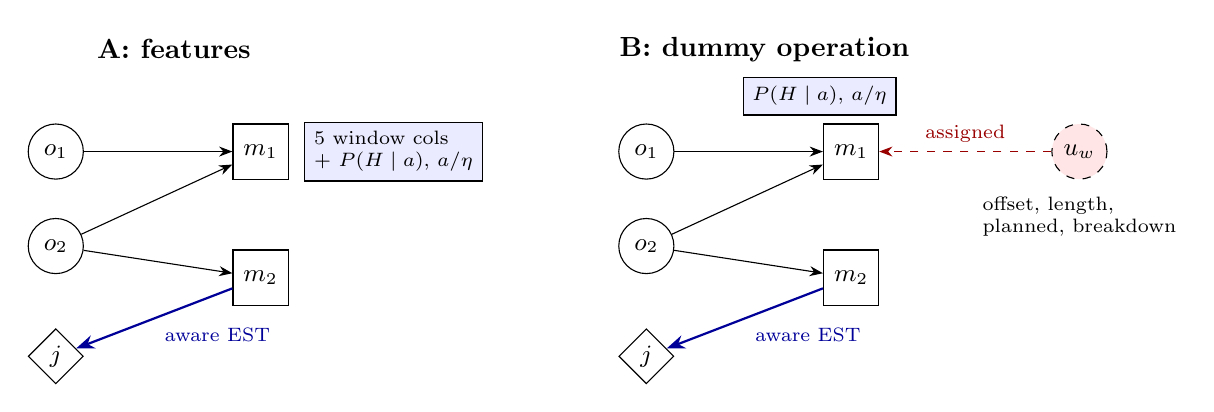
\begin{tikzpicture}[
  op/.style={circle,draw,minimum size=7mm,inner sep=0pt,font=\small},
  dum/.style={circle,draw,dashed,fill=red!10,minimum size=7mm,inner sep=0pt,font=\small},
  mach/.style={rectangle,draw,minimum size=7mm,font=\small},
  job/.style={diamond,draw,minimum size=7mm,inner sep=0pt,font=\small},
  feat/.style={rectangle,draw,fill=blue!8,font=\scriptsize,align=left},
  >=Stealth]
  % Representation A
  \node[font=\bfseries] at (1.5,2.3) {A: features};
  \node[op] (o1) at (0,1) {$o_1$};
  \node[op] (o2) at (0,-0.2) {$o_2$};
  \node[job] (j1) at (0,-1.6) {$j$};
  \node[mach] (m1) at (2.6,1) {$m_1$};
  \node[mach] (m2) at (2.6,-0.6) {$m_2$};
  \draw[->] (o1) -- (m1);
  \draw[->] (o2) -- (m2);
  \draw[->] (o2) -- (m1);
  \draw[->,thick,blue!60!black] (m2) -- node[below right,font=\scriptsize]{aware $\EST$} (j1);
  \node[feat,right=2mm of m1] {5 window cols\\+ $P(H\mid a)$, $a/\eta$};
  % Representation B
  \begin{scope}[xshift=7.5cm]
  \node[font=\bfseries] at (1.5,2.3) {B: dummy operation};
  \node[op] (p1) at (0,1) {$o_1$};
  \node[op] (p2) at (0,-0.2) {$o_2$};
  \node[job] (k1) at (0,-1.6) {$j$};
  \node[mach] (n1) at (2.6,1) {$m_1$};
  \node[mach] (n2) at (2.6,-0.6) {$m_2$};
  \node[dum] (u) at (5.5,1) {$u_w$};
  \draw[->] (p1) -- (n1);
  \draw[->] (p2) -- (n2);
  \draw[->] (p2) -- (n1);
  \draw[->,thick,blue!60!black] (n2) -- node[below right,font=\scriptsize]{aware $\EST$} (k1);
  \draw[->,dashed,red!60!black] (u) -- node[above,font=\scriptsize]{assigned} (n1);
  \node[font=\scriptsize,align=left,below=1mm of u] {offset, length,\\planned, breakdown};
  \node[feat,above=1mm of n1,xshift=-4mm] {$P(H\mid a)$, $a/\eta$};
  \end{scope}
\end{tikzpicture}
\caption{Where the window of machine $m_1$ is placed. In A it is five columns on $m_1$; in B it
is an operation node pre-assigned to $m_1$ that is never routed, queued or swapped. The
reliability columns and the window-aware action edges are identical in both. Buffer nodes
(\code{ojmb}) are omitted.}
\label{fig:reps}
\end{figure}

%=======================================================================
\section{Training with BOPO: common random numbers (point 7)}
\label{sec:crn}
%=======================================================================

\paragraph{How BOPO learns.} For one instance, BOPO samples a group of $B$ solutions with the
current policy, finds the best one (lowest makespan), and pairs it with the $K-1$ worst ones.
The loss then raises the probability of the best trajectory relative to the worse ones,
weighted by how much worse they are. The signal is purely comparative: \emph{this sequence of
decisions was better than that one}.

\paragraph{Why stochastic breakdowns break this.} If each rollout drew its own breakdowns, the
makespans in a group would differ for two reasons: the decisions, and the luck of the draw. A
rollout whose machines happened not to fail would be ranked best even if its decisions were
worse, and the policy would be trained to repeat them. Because makespan differences caused by
breakdowns are of the same order as those caused by decisions (windows cost about 20\% of the
makespan here), most of the preference signal would be noise.

\paragraph{Common random numbers.} Every rollout of a group faces the \emph{same} scenario: the
training environment draws one seed per group (\code{draw\_scenario}) and gives it to every
rollout copy (\code{fix\_scenario}) before they reset (\code{src/bopo.py}, \code{sample\_group}).
Within a group, the rollouts then differ only in their decisions, and the ranking measures what
it is meant to measure. Across groups a new scenario is drawn, so the policy still sees the
variability of the breakdowns during training. The scenario is sampled with a local
generator (\code{numpy.random.default\_rng(seed)}), never with the global random number
generators, so no other random draw (e.g.\ a sampled action) can change it. The test
\code{test\_bopo\_group\_shares\_the\_scenario} checks this through \code{sample\_group}.

\paragraph{Validation and test.} The validation and test splits store one realisation per
instance and mode, so every representation and every checkpoint is evaluated on exactly the
same windows, and comparisons between models are paired.

%=======================================================================
\section{References: clairvoyant bound under breakdowns (point 7)}
\label{sec:reference}
%=======================================================================

\subsection{CP-SAT model}

The blocking CP-SAT model is extended with the windows of each stored realisation. For every
operation $o$ and every eligible machine $m$ (presence literal $x_{om}$), with start $s_o$,
end of processing $c_o$ and departure $d_o$, each window $w$ of $m$ gets two Booleans: $a_w$
(the operation starts after $w$) and $y_w$ (its processing crosses $w$). The constraints,
enforced when $x_{om}$ holds, are
\begin{align*}
  a_w &\Rightarrow s_o\ge e_w, \qquad \neg a_w \Rightarrow s_o\le s_w-1 && \text{(R1)}\\
  \neg a_w &\Rightarrow s_o+p_{om}\le s_w \quad\text{if } \tau_w=\sch && \text{(R2)}\\
  y_w &\Leftrightarrow \neg a_w \wedge \Bigl(s_o+p_{om}+\sum_{w'<w}(e_{w'}-s_{w'})\,y_{w'}>s_w\Bigr) && \text{(R3)}\\
  c_o &= s_o+p_{om}+\sum_w (e_w-s_w)\,y_w, \qquad d_o\ge c_o \ (d_o=c_o \text{ for a job's last operation}).
\end{align*}
The occupancy interval $[s_o,d_o]$ stays in the machine's no-overlap constraint, and it is not
blocked by windows (R5). The horizon is the makespan of the window-aware earliest-completion
rule, and that rule's schedule is given as a starting solution. Without it, in a first test
CP-SAT found no schedule at all within 10\,s for a breakdown instance. Every CP-SAT schedule is checked with
the same constraint checks as the environment's schedules, so the solver and the environment
cannot silently disagree on R1--R5.

\subsection{Why it is a bound, not an optimum}

For scheduled windows the solver and the policy know the same windows, so the usual gap
$\RE=C_{\text{policy}}/C_{\text{CP-SAT}}-1$ is an optimality gap (up to CP-SAT's time limit).
With breakdowns, the solver is given the realised breakdowns \emph{in advance}. It can avoid a
machine that will fail, or finish an operation just before a failure, which no online policy
can do. Its makespan is a \emph{clairvoyant} (perfect-information) bound, and the gap to it
includes the unavoidable cost of not knowing the future. It is reported as \emph{gap to
clairvoyant}, never as an optimality gap. Only differences in this gap \emph{between
representations} are informative, since they share the same bound. The splits store the
reference per mode (\code{score\_scheduled}, \code{score\_breakdown}, \code{score\_mixed}), and
a model is scored against the mode it was trained on.

%=======================================================================
\section{Calibration}
%=======================================================================

As in the blocking study, the windows must bind, otherwise all three representations tie.
\code{src/calibrate\_unavailability.py} runs the earliest-completion rule on 10 instances of
the blocking setting for a grid of window settings. It compares the rule without windows,
window-blind, and window-aware, on the same realisations. The chosen setting (mixed mode) is:
\begin{center}
\begin{tabular}{@{}lr@{}}
\toprule
Measure (mean over 10 instances) & Value \\
\midrule
downtime cost: makespan with / without windows & 1.201 \\
share of machine time inside windows & 15.9\% \\
parts waiting in the buffer of a machine while it is down (per instance) & 9.7 \\
swaps / waits per instance & 1.2 / 0.3 \\
info value: window-blind / window-aware makespan of the greedy rule & 1.018 \\
\midrule
downtime cost, breakdowns only / scheduled only & 1.234 / 1.107 \\
\bottomrule
\end{tabular}
\end{center}

\begin{critique}{a greedy rule barely uses the windows}
Across the whole grid, the window-aware greedy rule is between 0.5\% worse and 3.5\% better
than the window-blind one. The two rules choose the same action in almost every decision. The earliest
completion over all jobs is rarely an option that a window delays, and the windows mostly change
the estimates of options that are not chosen anyway. Knowing the windows therefore pays only
with look-ahead: not trapping parts in the buffer of a machine that will soon be down, and
keeping work for the machines that will stay up. That is exactly what a learned policy with a
good representation can add. It also means that the expected differences between A, B and the
control are modest, and must be measured against the gap between the rule and CP-SAT, not
against the rule itself. This should be stated in the thesis before the results.
\end{critique}

%=======================================================================
\section{Experimental design}
\label{sec:design}
%=======================================================================

\begin{itemize}[nosep]
  \item \textbf{Representations}: \code{ojmb\_uf}, \code{ojmb\_uo} and \code{ojmb\_u0}
        (\code{main.py --representation unavailability}).
  \item \textbf{Modes}: \code{mixed} (main), and \code{scheduled} and \code{breakdown} separately.
        Scheduled only is the cleanest comparison (ordinary optimality gap); breakdown only
        isolates the reliability signal.
  \item \textbf{Blocking representation}: fixed to buffer nodes (\code{ojmb}). \code{ojmd}
        is supported (\code{blocking\_repr="dummy"}) but crossing both factors is not the
        research question.
  \item \textbf{Seeds}: at least 3 training seeds per cell. A one-seed difference between A and
        B is not evidence.
  \item \textbf{Evaluation}: \code{run\_metrics.py} on \code{val/test\_dataset\_unavailability.json},
        with paired tests on the same instances and realisations (Wilcoxon signed-rank, with
        effect sizes).
  \item \textbf{Metrics}: makespan and gap (to clairvoyant under breakdowns); interrupted time;
        \emph{trapped parts and trapped time} (parts waiting in the input buffer of a machine
        while it is down: the downtime-induced blocking cascade the representations target);
        swaps and waits; and all the existing efficiency and representation metrics.
\end{itemize}

\paragraph{Hypotheses (stated before the results).}
\begin{description}[nosep]
  \item[H1] \code{ojmb\_uf} and \code{ojmb\_uo} have a lower gap than \code{ojmb\_u0} in
            \code{scheduled} mode, because the information is useful when used with look-ahead.
  \item[H2] With parity by construction, A and B differ little. Any difference is due to
            structure: B's attention competition with real operations (in favour of A), and B's
            explicit reserved-capacity semantics (in favour of B).
  \item[H3] In \code{breakdown} mode, the representations beat the control mainly through the
            reliability columns, i.e.\ by routing away from old, unreliable machines. This shows
            as fewer trapped parts and less interrupted time.
  \item[H4] Representations that expose windows reduce trapped time, which is where the
            interaction with blocking appears.
\end{description}

%=======================================================================
\section{Remaining open points}
%=======================================================================

\begin{enumerate}[nosep]
  \item \textbf{Dedicated node type (C).} The blocking study contrasted a \emph{new node type}
        with an \emph{existing node type plus a flag}. This study contrasts \emph{features} with
        an \emph{existing node type plus a flag}. These are different axes, so the two studies
        cannot be merged into one conclusion (``dummy nodes are better or worse'') unless a
        \code{window} node type is added, or the text limits the claim.
  \item \textbf{Calendar-time ageing.} Age counts calendar time, not processing time. This keeps
        the scenario independent of the decisions, which common random numbers and fixed
        CP-SAT intervals require. The cost is that the policy cannot slow the ageing of a machine
        by loading it less. Usage-based ageing would be more realistic, but it needs a
        decision-dependent scenario and a different reference.
  \item \textbf{Weak binding in scheduled-only mode.} With the calibrated lengths, planned
        maintenance alone costs 10.7\% of makespan; longer windows (0.10--0.20 LB) cost
        19.3\%. If scheduled-only becomes the main comparison, the longer windows are
        preferable.
  \item \textbf{Reference cost.} 40 instances $\times$ 3 modes $\times$ 120\,s is about 4 hours
        of CP-SAT. With breakdowns, CP-SAT rarely proves optimality within the limit, so the
        references are incumbents and their status is stored.
\end{enumerate}

%=======================================================================
\section{Implementation map}
%=======================================================================

\begin{center}
\small
\begin{tabularx}{\textwidth}{@{}>{\raggedright\arraybackslash}p{0.38\textwidth} X@{}}
\toprule
File & Content \\
\midrule
\code{src/unavailability\_config.py} & chosen setting and calibration record \\
\code{src/unavailability.py} & $\EST$, resume, information view, $P_m(H\mid a)$, Weibull scenario sampler \\
\code{src/env\_unavailability.py} & environment: rules R1--R8, information model, representations A, B and control, normalisation, common random numbers \\
\code{src/env\_blocking.py} & \code{\_known\_end} hook (no change in behaviour) \\
\code{src/solver\_blocking.py} & CP-SAT windows (R1--R3, R5), horizon and hint \\
\code{src/metrics/unavailability.py} & independent checks and trapped / interrupted statistics \\
\code{src/bopo.py} & common random numbers in \code{sample\_group} \\
\code{src/generate\_unavailability\_}\newline\code{references.py} & validation / test splits with realisations and per-mode references \\
\code{src/calibrate\_unavailability.py} & calibration grid \\
\code{src/train.py}, \code{main.py},\newline\code{run\_metrics.py} & registration, per-mode scores, output folders \\
\code{tests/test\_}\newline\code{unavailability.py} & 12 tests (arithmetic, sampler, feasibility, leak, parity, normalisation, solver, common random numbers) \\
\bottomrule
\end{tabularx}
\end{center}

\end{document}
